% Chapter 4
\chapter{Solution}

\label{Chapter4} 
le Software-Defined Networking a rapidement émergé comme une technologie prometteuse pour les réseaux futurs et a gagné beaucoup d'attention. Cependant, la nature centralisée du SDN rend le système vulnérable aux attaques par déni de services (DoS), une fois le contôleur compris, tout le réseau cessera de fonctionner. Mais cette centralisation a un avantage, la gestion centralisée des équipements réseau, elle permet d'avoir une vue globale des flux de trafic, ce qui offre un meilleur système de défense contre les attaque DoS.\\

Comme mentioné dans la section \ref{rDoS}, nous nous intéréssons dans notre travail à une attaque DOS spécifique, connue sous le nom de \textbf{Reflective-DoS} (RDoS). Cette attaque est un peu spéciale est diffère carrément des autre types d'attaques DoS, dans le pricipe de fonctionnement et les dommages causés. On parlera plus sur cette attaque dans la section suivante. \\

Ce chapitre portera sur la conception de notre solution. Nous commençons par la problématique et la motivation de notre travail, suivi des hypothèses de conception. On passera après à la première étape de la conception, où on présentra l'architecture de notre système et ses différents composants. L'étape suivante est la contrustion de notre modèle de clustering  et terminera évidement avec une conclusion sur le travail efféctué.

\section{Problématique}
Mars 2018, un nouveau record a été marqué avec 1.7 TBps de traffic généré par une attque DoS réflective. La compagnie \textbf{Arbor Networks} a affirmé que son système d'analyse de trafic, ATLAS, a enregistré 1.7 Tbps d'une attaque reflective contre un site web d'un client[\cite{22}].\\

RDoS n’attaque pas directement la cible mais envoie plutôt plusieurs requête vers un service tiers exploitable (c.-à-d. le réflecteur, généralemnt c'est un serveur) avec une adresse IP d’expéditeur usurpée, ce qui rend l'attaquant anonymat. Les réponses du serveur tiers sont ensuite envoyés à la cible d’attaque réelle et causer une surcharge. Les protocoles avec des messages de réponse qui sont beaucoup plus grands que les messages de demande sont particulièrement bien adapté à ces attaques en raison des effets d’amplification. La nature de ces attaques nécessite des services qui fonctionnent sans connexion établie entre le client et le serveur. Une étude récente[\cite{23}] a trouvé que $ 99.72\% $ des attauqes RDoS utilisent des protocols basé UDP comme DNS, NTP, ..etc. Les messages reçus dans une attaque RDoS sont difficiles à différencier du trafic bénin, car ils sont conformes aux spécifications du protocole. Les réflecteurs sont correctement gèrent toutes les demandes comme légitimes, mais l’absence de réponses est une caractéristique des attaques réflective qui ne peut être masquée. 

\begin{figure}[h]
\centering
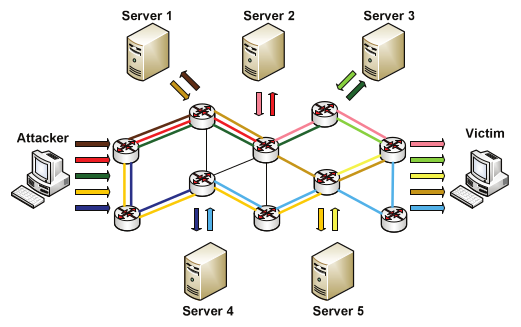
\includegraphics[width=0.7\textwidth]{Figures/rDoS}
\decoRule
\caption{Principe de dénie de service réflectif}
\label{fig:rDoS}
\end{figure} 

A ce niveau on peut clairement voir que l'impact de ce type d'attaque est en double; en premier lieu, la consomation de la bande passante des liens réseau à cause au nombre excesive des message, requêtes et réponses échnagés et deuxième lieu, la suchage des serveurs tiers avec des messages requêtes, qui vont les traiter évidement, car pour eux ils paraissent des requêts légitimes.\\
  
Pour cette fin, nous proposons une approche de clustering pour la détéction des d'attaque DoS réflectives dans un réseau SDN. Le but et de 

\section{Hypothèses}
Pour que notre système fonctionne de manière sûre et efficace, les hypothèses suivantes sont à prendre en considération :\\
\begin{itemize}
\item[•] Notre système est responsable de surveiller le réseau pour détecter uniquement les attaques de type DoS.\\
\item[•] On suppose que les liens entre le plan de données et le plan de contrôle sont fiables et dotés d’une bande passante suffisante pour faire circuler le trafic de contrôle nécessaire pour le fonctionnement du système et le protocole utilisé pour la communication entre ces deux plans est OpenFlow.\\
\item[•] Le réseau n’a pas été compromis avant ou durant le déploiement du système.\\
\item[•] Dernière hypothèse, qui est la plus importante. Notre modèle a été traîné sur le Dataset suivant xxxxxx. Tout résultat généré par ce système après son déploiement dépendra de cette Dataset.
\end{itemize}

\section{Architecture générale}


 